\chapter{Raspberry Piをリモコンにしてみよう}
\section{センサーの基本}
\subsection{センサーってなんだろう?}
センサーは身の回りの世界の情報を調べ、コンピュータに伝えるための装置です。明るさ、温度、湿度を調べることができるセンサーボードは第3回の授業で扱いました。しかし、センサーはたくさんの種類があり、出来ることももっとたくさんあります。まず、車で使われているセンサーを見てみましょう。

\begin{figure}[htb]
\begin{center}
    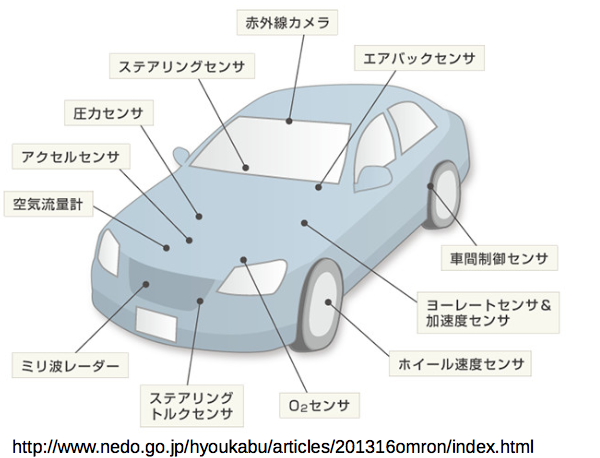
\includegraphics[scale=1.0]{images/chap05/text05-img001.png}
    \caption{自動車に使われているセンサー}
    \label{fig1}
\end{center}
\end{figure}

\begin{table}[htb]
  \centering
  \begin{tabular}{|l|l|} \hline
\multicolumn{1}{|c|}{センサーの種類} & \multicolumn{1}{c|}{できること} \\ \hline\hline
赤外線カメラ & 暗闇で物を見ることができる \\
ステアリングセンサ & ハンドルの回し具合によってタイヤの方向を決める \\
圧力センサ & 圧力を調べる \\
アクセルセンサ & アクセルペダルの踏み具合を調べる \\
ミリ波レーダー & 車の前に物があるかを調べる \\
トルクセンサ & ねじれの強さを調べる \\
$O_2$センサ & 燃料の働き具合を空気の酸素($O_2$)量で調べる \\
ホイール速度センサ & タイヤの回転速度を調べる \\
ヨーレートセンサ&加速度センサ & 車の速さを調べる \\
車間制御センサ & 前の車との距離を調べる \\
エアバックセンサ & 車の衝突を感知して瞬時にエアバッグを膨らませる \\ \hline
  \end{tabular}
\end{table}

このように、機械では多くのセンサーが使われています。今日の授業ではセンサーをいくつか扱います。どのセンサーが何に使えそうか、何に使われていそうかを考えながら使ってみましょう。

\begin{tcolorbox}[title=\useOmetoi]
\begin{enumerate}
\addquiz{センサーとはなんだろう。説明してみよう。}
\end{enumerate}
\end{tcolorbox}
\begin{tcolorbox}[title=\useOmetoi]
\begin{enumerate}
\addquiz{車で使われているセンサーを3つ書いてみよう。}
\end{enumerate}
\end{tcolorbox}

\subsection{アナログ信号とデジタル信号}
センサーが出力するデータは大きく分けて2種類あり、デジタル信号とアナログ信号と呼ばれる信号のどちらを使うかで分けられています。2つの信号には以下の図のような違いがあります。

\begin{figure}[htbp]
  \begin{minipage}[b]{0.45\linewidth}
    \centering
    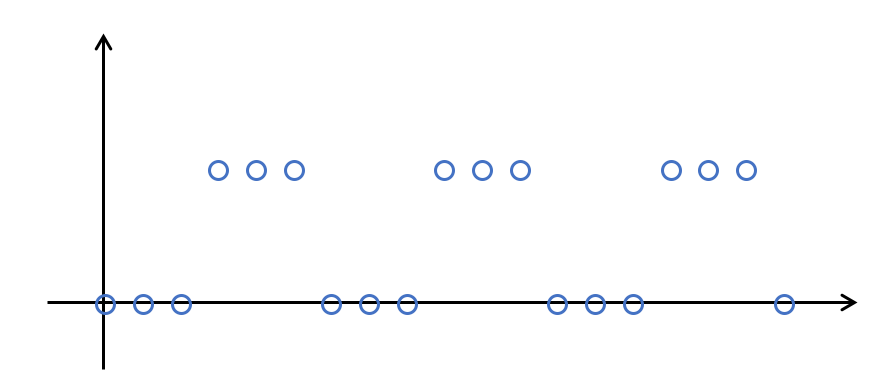
\includegraphics[keepaspectratio, scale=0.4]{images/chap05/text05-img002.png}
    \caption{デジタル信号の例}
    \label{fig2}
  \end{minipage}
  \begin{minipage}[b]{0.45\linewidth}
    \centering
    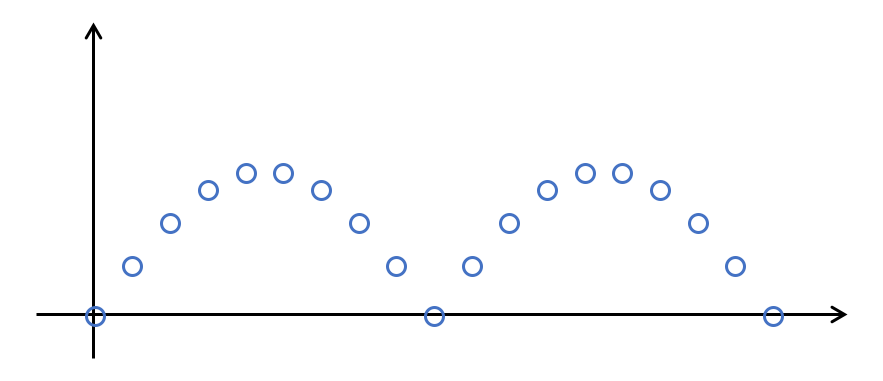
\includegraphics[keepaspectratio, scale=0.4]{images/chap05/text05-img003.png}
    \caption{アナログ信号の例}
    \label{fig3}
  \end{minipage}
\end{figure}

図\ref{fig2}と図\ref{fig3}はコンピュータで使われている信号をグラフにしたものです。授業で使用するセンサーのデジタル信号は、図\ref{fig2}と図\ref{fig3}のように2種類の値を表すことができます。2種類の値は0か1です。一方授業で使用するアナログ信号は、\ref{fig3}のように中間の値を表すことができます。この値は0〜1023の数字で表現されます。

デジタル信号はボタンが押されたか押されていないか、明かりがついたか消えたかなどのふた通りのものを表すときに使われ、アナログ信号は主に明るさや距離などの数を表すときに使われます。

\begin{tcolorbox}[title=\useOmetoi]
\begin{enumerate}
\addquiz{アナログ信号、デジタル信号の違いを書いてみましょう。}
\end{enumerate}
\end{tcolorbox}